\documentclass[11pt]{article}
\usepackage{graphicx}
\usepackage{times}
\pagestyle{myheadings}
\def\dot{{\sc dot}}
\def\dotty{{\sc dotty}}
\def\neato{{\sc neato}}
\newcommand{\lastedited}{April 26, 2004}
\date{\lastedited}
\newcommand{\mymark}{\hfil \neato\ User's Manual, \lastedited \hfil}
\markboth{\mymark}{\mymark}
\begin{document}
\bibliographystyle{alpha}
% \keywords{Graph Layout, Network Visualization, Graph Browser}
\title{Drawing graphs with \neato}
\author{Stephen C. North}
\maketitle
\begin{abstract}
\noindent
\neato\ is a program that makes layouts of undirected graphs
following the filter model of \dot.
Its layout heuristic creates virtual physical models and runs an
iterative solver to find low energy configurations.
The intended applications are in telecommunication networks,
computer programming and software engineering.
Here is an example layout depicting an entity-relationship
database schema.  It took 0.01 seconds of user time to generate
on a garden variety PC running Linux. 
\par
\vspace*{.25in}
\centerline{ 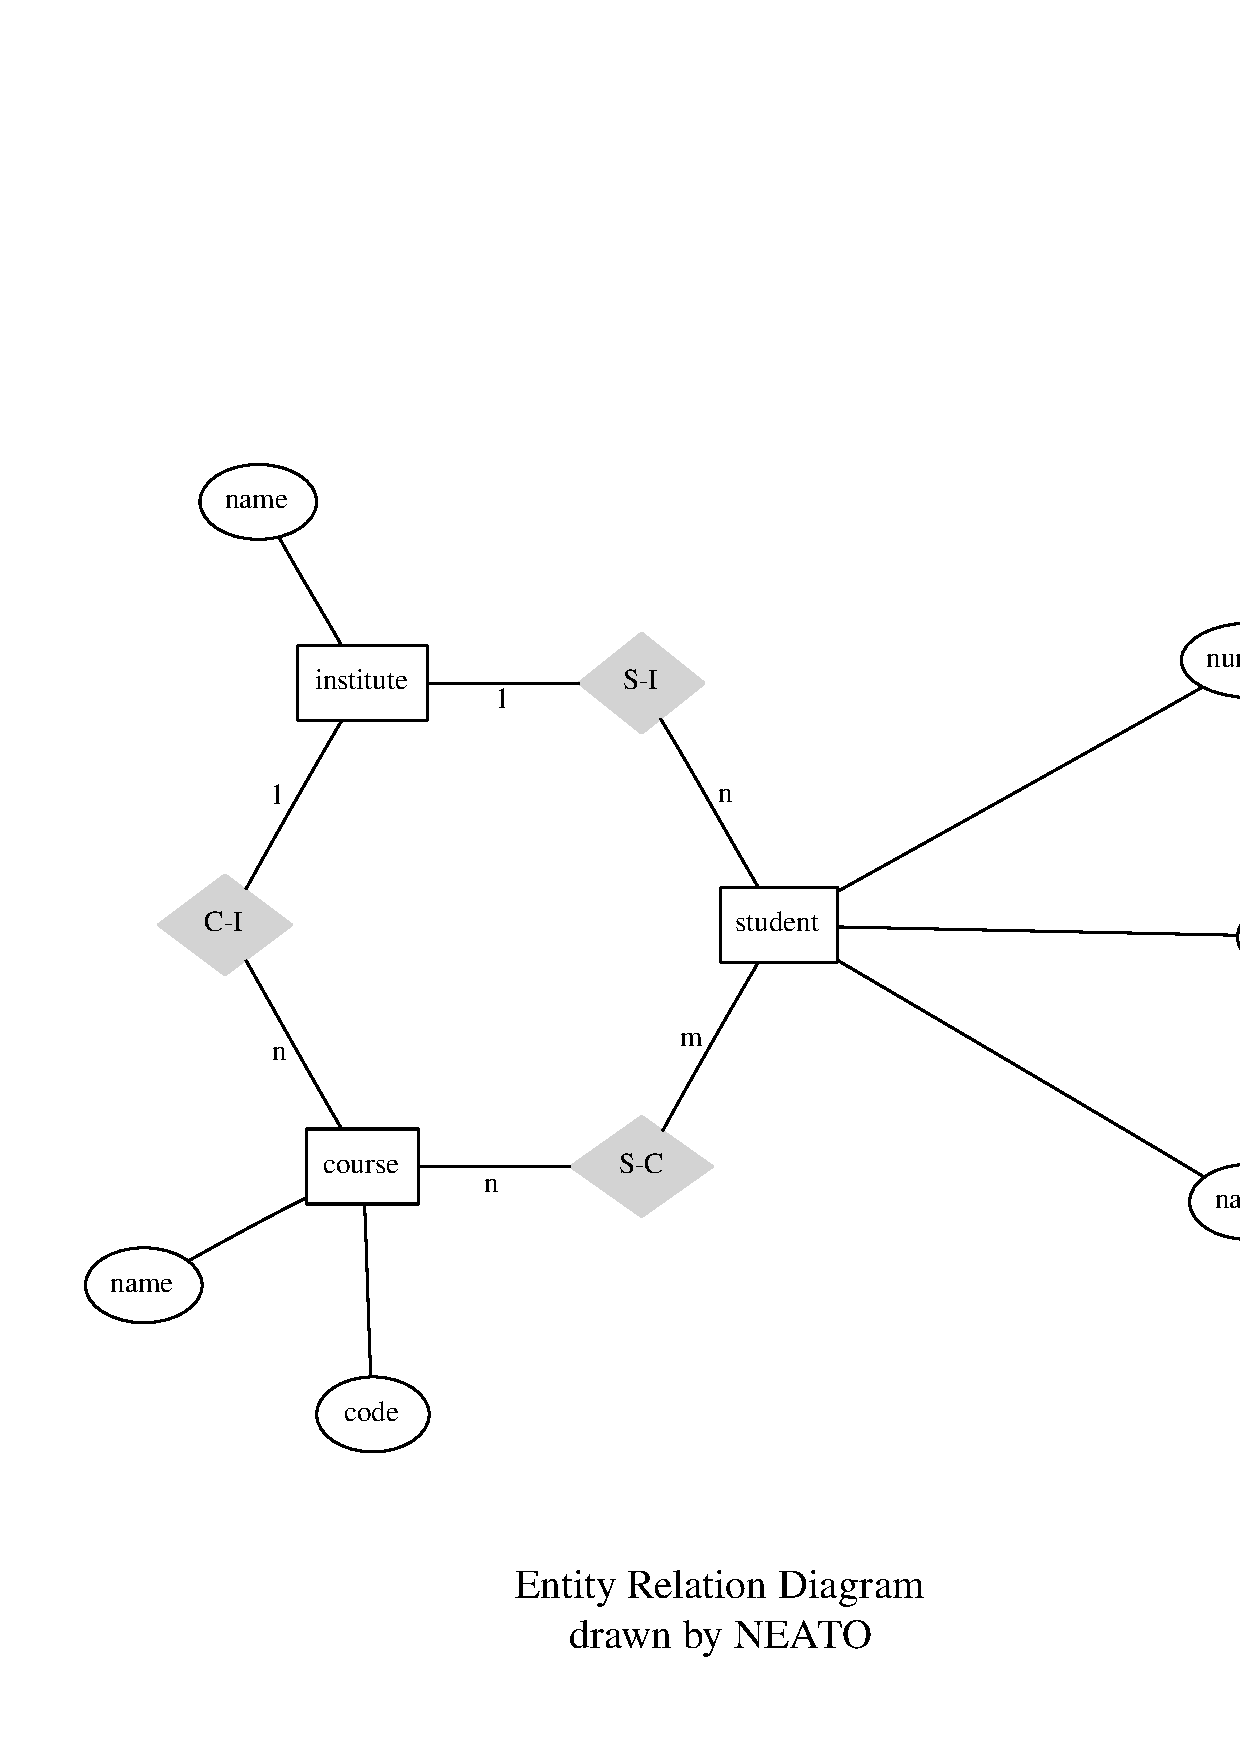
\includegraphics{ER} }
\end{abstract}

\newpage
\section{Introduction}
\neato\ is a utility that draws undirected graphs,
which are common in telecommunications and computer programming.
It draws a graph by constructing a virtual physical model
and running an iterative solver to find a low-energy configuration.
Following an approach proposed by Kamada and Kawai \cite{kk},
an ideal spring is placed between every pair of nodes such that
its length is set to the shortest path distance between the endpoints.
The springs push the nodes so their geometric distance in the layout
approximates their path distance in the graph.
This often yields reasonable layouts \cite{spremb}\cite{reingold-fructerman}.
(In statistics, this algorithm is also known as multidimensional scaling.
Its application to graph drawing was noted by Kruskal and Seery in the
late 1970s.)
\begin{figure}[b]
\begin{minipage}[b]{2in}
\begin{verbatim}
graph G {
    run -- intr;
    intr -- runbl;
    runbl -- run;
    run -- kernel;
    kernel -- zombie;
    kernel -- sleep;
    kernel -- runmem;
    sleep -- swap;
    swap -- runswap;
    runswap -- new;
    runswap -- runmem;
    new -- runmem;
    sleep -- runmem;
}
\end{verbatim}
\end{minipage} \hspace{.5in} \
\parbox[b]{2.5in}{
	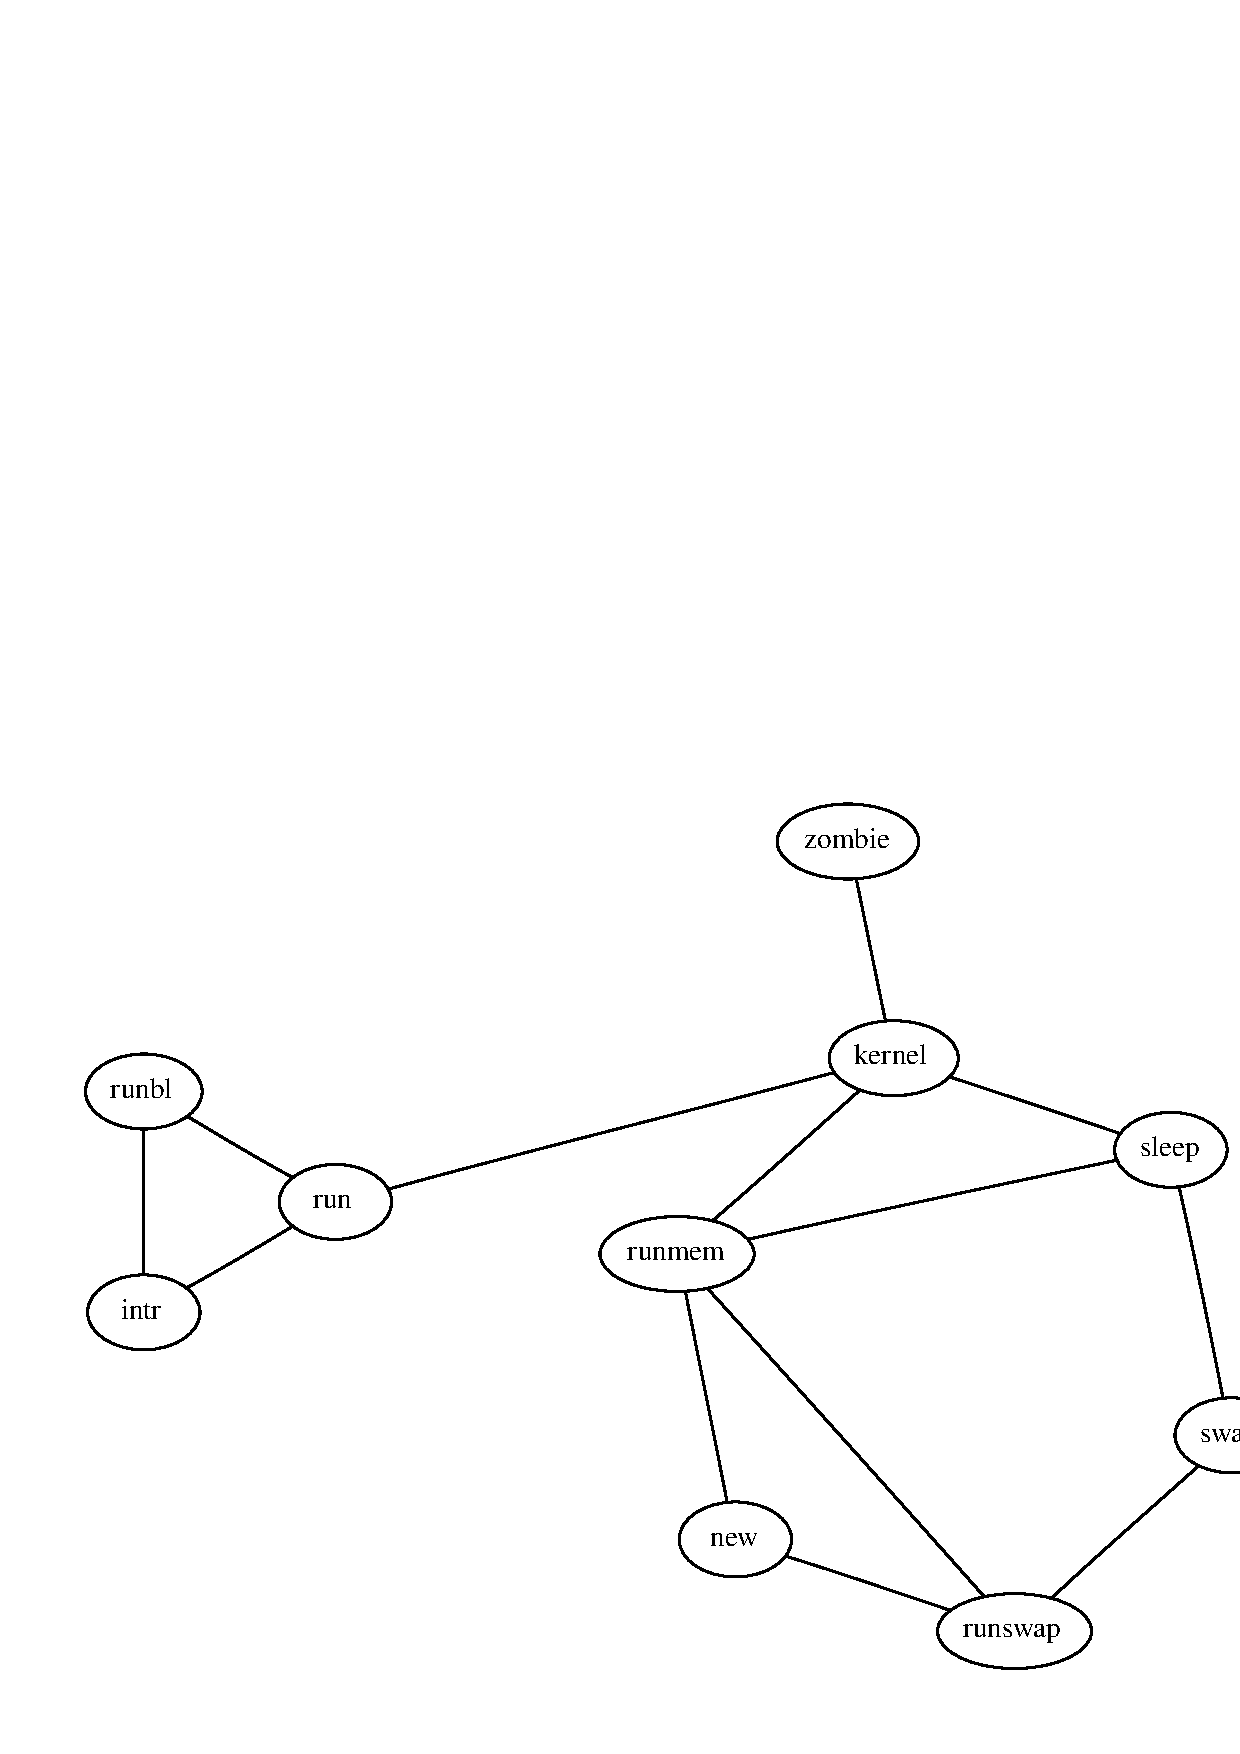
\includegraphics[scale=.6]{process}
}
\caption{Process States in an Operating System Kernel (0.03 seconds)}
\label{fig:process}
\end{figure}

\neato\ is compatible with the directed graph drawing program
\dot\ in sharing the same input file format
and graphics drivers \cite{dotuserguide}.
Since the file format includes both undirected and directed graphs,
\neato\ draws graphs prepared for \dot, and vice versa.
Both programs have the same options for setting labels, colors, shapes,
text fonts, and pagination, and for generating code in common graphics
languages (PostScript, raster formats such as GIF and PNG, SVG,
FrameMaker MIF, and web click maps).
Both work with \dotty, an interactive graph viewer for X windows.
(The {\tt lneato} command script runs neato from an interactive window.)

Figs.~\ref{fig:process}--\ref{fig:IMR} are representative 
examples of \neato's output.
The timings refer to user time on a 600 Mhz Pentium Linux server.
Fig.~\ref{fig:process} was derived from a hand-made drawing
in an operating system tutorial.
Fig.~\ref{fig:inet} shows the connectivity of a computer network.
Fig.~\ref{fig:typesharing} shows the sharing of programmer-defined types
between procedures in a C program.  The program that was the source
of this graph parses a text file into an internal data structure.
The graph was extracted from a C program database.  Its drawing shows
where interactions or conversions between types may occur.  Finally,
Fig.~\ref{fig:IMR} shows relationships between IMRs (modification requests)
in an externally released software product.\footnote{Graph
courtesy of J. Hoshen, Bell Labs.} The labeled nodes are IMRs and the small circles
encode many-to-many dependencies.
\begin{figure}[h]
	\centerline{\includegraphics{inet}}  % y=4in
	\vspace{.25in}
    \caption{R\&D Internet Backbone (0.08 seconds)}
    \label{fig:inet}
\end{figure}

\begin{figure}[h]
	\centerline{\includegraphics{typeshar}} % xsize=4in
    \caption{Type Sharing Between Procedures in a C Program (0.41 seconds)}
    \label{fig:typesharing}
\end{figure}
\begin{figure}[h]
	\centerline{\includegraphics{jho}}  %xsize=4in
	\caption{IMR Dependencies (6.75 seconds)}
	\label{fig:IMR}
\end{figure}
\clearpage

\begin{figure}[h]
\begin{minipage}[b]{2in}
\begin{verbatim}
$ cat example.gv
graph G {
    n0 -- n1 -- n2 -- n3 -- n0;
}
$ neato -Tps example.gv -o example.ps


\end{verbatim}
\end{minipage} \hspace{1.0in} \
\parbox[b]{2.5in}{
	\ \\
    \centerline{\includegraphics{G4_orig}}
}
\caption{Example Graph Drawing}
\label{fig:G4_orig}
\end{figure}

\section{Graph Drawing}
\subsection{Basic Commands}
The remainder of this memo gives a synopsis of \neato\ features.
Many of these should be familiar to users of \dot.
Fig.~\ref{fig:G4_orig} shows a graph file, its drawing,
and the command that was executed. A graph file has a
short header and a body consisting of nodes, edges, and
attribute assignments.
By default, nodes are drawn as ellipses labeled with node names.
Undirected edges are created by the \verb"--" operator.
Edges are drawn as straight lines and tend to be all about the same length.

\subsection{Drawing Options}
Table~\ref{table:attrs} lists the graph, node and edge
attributes that affect the layout.
The options to set labels, shapes, fonts, and sizes are convenient
for many kinds of layouts.  The drawing in figure~\ref{fig:fancy}
illustrates some of these features.\footnote{Graph courtesy of
Hector Zamora, DEFINITY.}
Options to set the size of the drawing, pagination, and output graphics
language are also the same as in \dot.

\begin{figure}
	\centerline{\includegraphics{fancy}}	 % ysize=5
\footnotesize
\begin{verbatim}
graph G {
        node [shape=box,style=filled];
        {node [width=.3,height=.3,shape=octagon,style=filled,color=skyblue] A1 A2 A3}
        A -- A1 [label="l #6"];
        A -- A2 [label="l #7"];
        A -- A3 [label="l #8"];

        {edge [style=invis]; A1 -- A2 -- A3}

        edge [len=3];   /* applies to all following edges */
        A -- B [label="l #1"]; A -- C [label="l #2"]; A -- D [label="l #3"];
        A -- E [label="l #4"]; A -- F [label="l #5"]; B -- C [label="l #1"];
        B -- E [label="l #2"]; B -- F [label="l #3"]; C -- D [label="l #1"];
        D -- E [label="l #1"];
}
\end{verbatim}
    \caption{Node and Edge Options}
    \label{fig:fancy}
\end{figure}

\section{Adjusting Layouts}
Although layouts made by \neato\ are close to a local optimum
as defined by the forces the springs exert on the nodes,
fine tuning or generation of alternative layouts may improve readability.
Because \neato\ uses unconstrained optimization, it does not enforce
minimum separation constraints between nodes or between edges and
nonadjacent nodes, so in dense graphs nodes and edges can be too
close or overlap.  There are three ways of trying to correct these errors:
\begin{obeylines}
1) change the initial configuration
2) adjust the solver parameters
3) edit the input edge lengths and weights.
\end{obeylines}

\subsection{Initial Configuration}
If no options are given,
\neato\ always makes the same drawing of a given graph file,
because its initial node placement and the solver are deterministic.
Random initial placement can yield different layouts.
It is sometimes reasonable to make at least several different
trial layouts, and accept the best one.
Random initial placement is requested by setting the value of the
graph attribute \verb"start".
If the value is a number, it is taken as a seed for the random number
generator. The layout is different for each seed, but still deterministic.
If the value is not a number, the process ID or current time is used.
Each run potentially yields a different drawing.  For example:
\begin{verbatim}
$ neato -Tps -Gstart=rand file.gv > file.ps
\end{verbatim}

\subsection{Termination Threshold}
The solver is a Newton-Raphson algorithm that moves a node
with a maximal $\delta e$ on every iteration.
The solver terminates when $\delta e$ falls below some $\epsilon$.
The default ($.1$) is low enough that the layout is usually
close to a local minimum, but not so low that the solver runs
for a long time without making significant progress.
Smaller values of $\epsilon$ allow the solver run longer and 
potentially give better layouts.  Larger values can decrease
\neato's running time but with a reduction in layout quality.
This may be a desirable tradeoff for large graphs.
$\epsilon$ is set in the graph's \verb"epsilon" variable.
You can also directly limit the number of iterations.
It is convenient to do this on the command line:
\begin{verbatim}
$ neato -Tps -Gepsilon=.001 small.gv -o small.ps
$ neato -Tps -Gepsilon=1.5 big.gv -o big.ps
$ neato -Tps -Gmaxiter=1000 big.gv -o big.ps
\end{verbatim}

\subsection{Edge Lengths and Weights}
Since the layout depends on the input edge lengths and their weights,
these can sometimes be adjusted to good effect.
The length of an edge is the preferred distance between the endpoint nodes.
Its weight is the strength of the corresponding spring, and affects the cost
if it is stretched or compressed.  Invisible edges can also be inserted to
adjust node placement.  In figure~\ref{fig:fancy}, the length of some
edges was set to 3 to make them longer than the default.
Also, the two invisible edges affect A1, A2, and A3.

There is also a way to also give the initial or final coordinates of
individual nodes.  The initial position, formatted as two comma-separated
numbers, is entered in a node's \verb"pos" attribute.  If \verb"!" is given
as a suffix, the node is also pinned down.

\begin{figure}
\begin{minipage}[b]{2in}
\begin{verbatim}
graph G {
        n0 -- n1 [len=2, style=bold];
        n1 -- n2 -- n3 -- n0;
}

\end{verbatim}
\end{minipage} \hspace{1.0in} \
\parbox[b]{2.5in}{
	\ \\
    \includegraphics{G4_lenwt}
}
\caption{Example graph with an edge stretched}
\label{fig:G4_lenwt}
\end{figure}

\begin{figure}
\begin{minipage}[b]{2in}
\begin{verbatim}
graph G {
    n0 [ pos = "0,0!" ];
    n1 [ pos = "2,0" ];
    n2 [ pos = "2,2!" ];
    n0 -- n1 -- n2 -- n3 -- n0;
}


\end{verbatim}
\end{minipage} \hspace{.5in} \
\parbox[b]{3in}{
	\ \\
    \includegraphics{G4_pinned}
}
\caption{Example graph with nodes pinned}
\label{fig:G4_pinned}
\end{figure}

\begin{table}
\begin{tabular}[t]{|l|l|p{3.5in}|} \hline
Name & Default & \hfil Values \hfil \\ \hline
\multicolumn{3}{|c|}{Node Attributes} \\ \hline
{\tt shape} & {\tt ellipse} & {\tt ellipse}, {\tt box}, {\tt circle}, {\tt doublecircle}, {\tt diamond}, {\tt plaintext}, {\tt record}, {\tt polygon} \\
{\tt height},{\tt width} & {\tt .5,.75} & height and width in inches \\
{\tt label} & node name & any string \\
{\tt fontsize} & {\tt 14} & point size of label \\
{\tt fontname} & {\tt Times-Roman} & font family name, e.g. {\tt Courier, Helvetica} \\
{\tt fontcolor} & {\tt black} & type face color \\
{\tt style} & & graphics options, e.g. {\tt bold, dotted, filled} \\ 
{\tt color} & {\tt black} & node shape color \\ 
{\tt pos} & & initial coordinates (append {\tt !} to pin node) \\ \hline
\multicolumn{3}{|c|}{Edge Attributes}   \\ \hline
{\tt weight} & {\tt 1.0} & strength of edge spring \\
{\tt label} & & label, if not empty \\
{\tt fontsize} & {\tt 14} & point size of label \\
{\tt fontname} & {\tt Times-Roman} & font family name \\
{\tt fontcolor} & {\tt black} & type face color \\
{\tt style} & & graphics options, e.g. {\tt bold, dotted, dashed} \\ 
{\tt color} & {\tt black} & edge stroke color \\
{\tt len} & 1.0 & preferred length of edge \\
{\tt dir} & {\tt none} & {\tt forward}, {\tt back}, {\tt both}, or {\tt none} \\ 
{\tt decorate} & & if set, draws a line connecting labels with their edges \\
{\tt id} & & optional value to distinguish multiple edges \\ \hline
\multicolumn{3}{|c|}{Graph Attributes}  \\ \hline
{\tt start} & & seed for random number generator \\
{\tt size} & & drawing bounding box, in inches \\
{\tt page} & & unit of pagination, {\it e.g.} {\tt 8.5,11} \\
{\tt margin} & {\tt .5,.5} & margin included in {\tt page} \\
{\tt label} & & caption for graph drawing \\
{\tt fontsize} & {\tt 14} & point size of label \\
{\tt fontname} & {\tt Times-Roman} & font family name \\
{\tt fontcolor} & {\tt black} & type face color \\ 
{\tt orientation} & {\tt portrait} & may be set to {\tt landscape} \\ 
{\tt center} & & when set, centers drawing on {\tt page} \\ \hline
{\tt overlap} & true & may be set to {\tt false} or {\tt scale} \\ \hline
{\tt splines} & false & {\tt true} makes edge splines if nodes don't overlap \\ \hline
{\tt sep} & 0 & edge spline separation factor from nodes - try .1 \\ \hline
\end{tabular}
\caption{Drawing attributes}
\label{table:attrs}
\end{table}

\section{Eliminating Overlaps}
To improve clarity, it is sometimes helpful to eliminate 
overlapping nodes or edges. One way to eliminate node overlaps
is just to scale up the layout (in terms of the center points
of the nodes) as much as needed.  This is enabled by setting
the graph attribute {\tt overlap=scale}.  This transformation
preserves the overall geometric relationships in the layout,
but in bad cases can require high scale factors.  Another way
to eliminate node overlaps employs an interative heuristic.
On each iteration, a bounded Voronoi diagram of the node center points
is computed, and each node is moved to the center of its Voronoi cell.
This is repeated until all overlaps are eliminated.  A side-effect
(perhaps unwanted) is that the adjusted layout tends to fill the
bounding rectangle of the Voronoi diagram.  The heuristic is activated
by setting {\tt overlap=false}.

Edge overlaps (with nodes) can be prevented by drawing them
with spline curves (with {\tt splines=true}). Note that the spline
drawing heuristic is expensive and probably should not be attempted
on graphs that have more than a few dozen nodes.

Areas for future work include non-rectangular Voronoi boundaries,
faster edge routing heuristics, and techniques to prevent
unnecessary edge intersections.

\section{Acknowledgments}

\neato's layout heuristic follows the work of Kamada and Kawai \cite{kk}.
The implementation was originally part of the {\sc salem} 3D viewer
for mathematical structures written with David Dobkin and Nathaniel Thurston.
In converting \neato\ to a more traditional tool, the graphics code generator
was borrowed from \dot.  This includes code contributed by John Ellson and
Emden Gansner.  Steve Eick was an early user and offered some good
suggestions about ways to adjust layouts.  Emden Gansner also contributed
the heuristics for eliminating node overlaps, based on a paper by
David Rappaport and Kelly Lyons.

\small
\bibliography{../dotguide/graphdraw} 
\end{document}
